\documentclass[a4paper]{article}

\usepackage{tecnico_relatorio}

\usepackage{textcomp}
\usepackage[hypcap]{caption} % makes \ref point to top of figures and tables
%\usepackage{rotating}
\usepackage{float}
\usepackage[]{tocbibind}

\begin{document}
	\trSetImage{img/tecnico_logo}{6cm} % Logotipo do Técnico
	\trSetSubject{Co-Projecto HW/SW}
	\trSetType{Parte I}
	\trSetTitle{Compressão de Texto Usando Codificação de Huffman}

	\trSetBoxStyle{0.3}

	\trSetAuthorNr{2}

	\trSetAuthors
		{
		\begin{center}
		Gonçalo Ribeiro

		73294
		\end{center}
		}{
		\begin{center}
		Luís Fiolhais

		74171
		\end{center}
		}

	\trSetProfessor{Prof. Horácio Neto}

	\trMakeCover

	\tableofcontents
	\pagenumbering{gobble}

  \pagebreak

  \pagenumbering{arabic}
  \setcounter{page}{1}


	\section{Introdução}

	\paragraph{} Nesta parte do trabalho pretende-se criar um sistema constituído por um único processador MicroBlaze e um acelerador por hardware. O tema escolhido para o projecto é compressão de texto usando codificação de Huffman.

	Inicialmente começou-se por implementar o algoritmo de compressão em software. Depois de verificada a sua funcionalidade, o seu desempenho foi medido incluindo \textit{AXI timers} no sistema e contabilizando o tempo despendido por cada parte do algoritmo para diversos ficheiros de exemplo. Com base nesta medição, escolheu-se uma parte do algoritmo para ser acelerada por hardware.

	O componente de hardware desenvolvido liga-se ao MicroBlaze através de uma interface FSL (\textit{Fast Simplex Link}). O acelerador foi desenhado e testado no Xilinx ISE (\textit{Integrated Synthesis Environment}) e subsequentemente integrado no sistema. O sistema foi testado e o desempenho foi novamente medido.

  Neste relatório apresentamos os resultados obtidos com aceleração e sem aceleração, tal como os problemas encontrados e áreas que ainda podem ser melhoradas.


	\section{Codificação de Huffman}
	\label{sec:theory}

	\paragraph{} A codificação de Huffman é um método de compressão que consiste em encontrar uma representação alternativa --- um \emph{código} --- para cada \emph{símbolo} do alfabeto dos dados a comprimir. A compressão resulta do facto de o código escolhido para um dado símbolo ser tanto mais curto quanto maior for a frequência absoluta desse símbolo nos dados. A símbolos mais raros são atribuídos códigos mais longos. Os códigos encontrados têm uma propriedade importante: nenhum código é prefixo de outro código. Isto permite que durante o processo de descompressão não haja qualquer ambiguidade.

	Os passos necessários ao algoritmo de compressão são os seguintes:

	\begin{enumerate}
	\item obter as frequências absolutas de cada símbolo
	\item construir uma árvore de Huffman
	\item codificar os dados
	\end{enumerate}

	O primeiro passo consiste em contar o número de ocorrências de cada símbolo até encontrar o fim do ficheiro. O segundo passo é criar uma \emph{trie} a partir das frequências obtidas no primeiro passo. Por último o ficheiro é comprimido fazendo uso da árvore criada.

	O processo de criação da árvore de Huffman é:

	\begin{enumerate}
	\item criar um nó para cada símbolo do alfabeto, em que se inclui a frequência desse símbolo
	\item enquanto existir mais que uma árvore
		\begin{enumerate}
		\item encontrar as duas árvores cuja raiz tem menor frequência
		\item tornar essas árvores descendentes de um novo nó, cuja frequência é a soma das frequências das raízes das duas árvores
		\end{enumerate}
	\end{enumerate}

	No final sobra apenas uma árvore que contém os nós correspondentes a cada símbolo. A localização desses nós na \textit{trie} dá-nos o código desse símbolo.

	\subsection*{Exemplo}

	\paragraph{} Tome-se como exemplo o ficheiro \texttt{ABBCCCDDDD<EOF>}, em que \texttt{<EOF>} é o carácter terminador do ficheiro. As estatísticas do ficheiro são as seguintes: \texttt{\{A: 1, B: 2, C: 3, D: 4, <EOF>: 1\}}. A partir das estatísticas retiradas do ficheiro é gerada uma lista de prioridade. Na \autoref{fig:prio_list} apresenta-se a lista obtida.

  \begin{figure}[H]
    \centering
    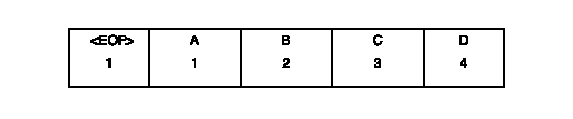
\includegraphics[width=.65\textwidth]{img/prio_list}
    \caption{Lista de prioridade gerada a partir das estatísticas}
    \label{fig:prio_list}
  \end{figure}

  De seguida retira-se os 2 elementos de menor prioridade da lista - neste caso \texttt{A} e \texttt{<EOF>} - e cria-se um novo nó que guarda a soma das suas frequências.

  \begin{figure}[H]
    \centering
    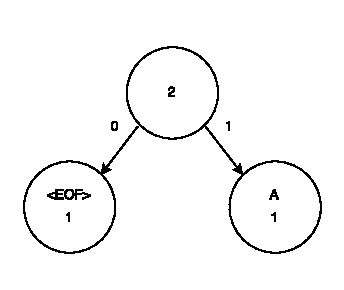
\includegraphics[width=.5\textwidth]{img/trie_1}
    \caption{Primeiro nó da árvore}
    \label{fig:trie_1}
  \end{figure}

  O novo nó vai ser adicionada à lista de prioridades, vamos chamar-lhe \texttt{Nó 1}.

  \begin{figure}[H]
    \centering
    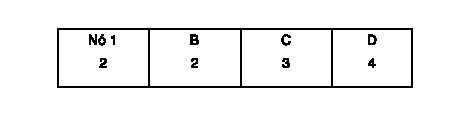
\includegraphics[width=.65\textwidth]{img/prio_list_2}
    \caption{Lista de prioridade com \texttt{Nó 1} adicionado}
    \label{fig:prio_list_2}
  \end{figure}

  Este processo repete-se até só existir um elemento na lista de prioridade. Na \autoref{fig:final_huffman_tree_example} pode ver-se a árvore de Huffman final criada para este ficheiro.

	\begin{figure}[H]
		\centering
		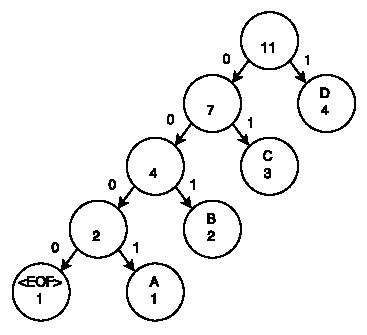
\includegraphics[width=.65\textwidth]{img/huffman_tree_example}
		\caption{Exemplo de uma árvore de Huffman}
		\label{fig:final_huffman_tree_example}
	\end{figure}

	Os códigos para cada carácter obtêm-se percorrendo a \textit{trie} da raiz até à folha que contem o respectivo carácter. Cada vez que se passa para um filho à esquerda adicionamos o bit 0 à codificação; cada vez que se segue para um filho à direita adiciona-se um bit com o valor 1. Assim, por exemplo o código de \texttt{A} é \texttt{0001}, o de \texttt{C} é \texttt{01} e o de \texttt{D} é \texttt{1}. É de notar que, tal como previsto, os caracteres que ocorrem menos vezes têm códigos mais curtos.

	O ficheiro comprimido seria portanto \texttt{0001 001 001 01 01 01 1 0000}. De $11 \times 8 = 88$ bits - assumindo que é usada a representação ASCII - passou-se a 21 bits.

	No entanto, seria ainda necessário colocar no ficheiro uma representação da árvore para que o ficheiro pudesse ser descomprimido. A árvore poderia ser representada no ficheiro de saída como \texttt{00001 <EOF> 1 A 1 B 1 C 1 D}, em que \texttt{A}, \texttt{B}, \texttt{C}, \texttt{D} e \texttt{<EOF>} representam a codificação original do caracteres em ASCII. Assim, na realidade o ficheiro comprimido teria neste caso $21 + 9 + 5 \times 8 = 70$ bits, obtendo-se um rácio de compressão de $79,5\%$. Em ficheiros pequenos a inclusão da árvore tem um grande impacto, como se percebe por este exemplo. Em ficheiros grandes o \textit{overhead} da inclusão da árvore é desprezável.

	\section{Software}

	\paragraph{} Nesta secção é descrita a implementação por software.

	\subsection{Estatísticas do Ficheiro}

	\paragraph{} Para obter a frequência absoluta de cada carácter do ficheiro é feito um varrimento do ficheiro e incrementado um contador relativo ao número de ocorrências desse carácter. Isto é feito até que seja encontrado o carácter terminador. Esse carácter está definido no programa como \texttt{FILE\_END\_CODE}. Ao longo desta parte do trabalho tem-se considerado como terminador o carácter \texttt{0x00}.

	A razão pela qual é preciso escolher um carácter como terminador prende-se com o facto de não termos um sistema operativo a correr no MicroBlaze. Caso tivéssemos um sistema operativo ele podia notificar o programa quando não houvesse mais conteúdo para ler.

	A complexidade desta fase do algoritmo é linear com o tamanho do ficheiro. Antes de se passar à construção da árvore, é construído um vector com pares (carácter, contagem), que não inclui caracteres com frequência absoluta nula. Na construção da árvore são portanto considerados apenas caracteres com pelo menos uma ocorrência. Isto resulta numa árvore mais pequena (menor \textit{overhead} no ficheiro comprimido) e torna a construção da árvore mais rápida.

	\subsection{Árvore}

	\paragraph{} Tal como visto na Secção~\ref{sec:theory} uma operação muito frequente durante a construção da árvore de Huffman é encontrar as duas raízes que em cada momento têm menor frequência absoluta. De forma a acelerar estas procuras, fez-se a implementação da árvore recorrendo a um acervo (\textit{heap}) que contém apontadores para os nós da árvore. O acervo é construído com complexidade $O(n)$, permite remoção do elemento com menor frequência em $O(log\ n)$ e inserção também $O(n)$, em que $n$ é o número de elementos, sendo que neste caso temos $n \leq 256$.

	Por cada dois elementos (nós) que são removidos do acervo é adicionado um novo com frequência igual à soma das frequências dos que foram removidos. Os nós removidos são depois ``pendurados'' debaixo do novo nó. Assim sendo, cada elemento do acervo é na verdade uma árvore. Quando o acervo tiver apenas um elemento temos certeza de que esse constitui a árvore de Huffman. Note-se que por cada dois elementos que são removidos é adicionado apenas um, pelo que construir a árvore de Huffman demora, no máximo, 255 passos.

	\subsection{Ficheiro de Saída}

	\paragraph{} Percorrendo a árvore de Huffman é possível obter o código que corresponde a cada carácter. De forma a optimizar o processo de codificação do ficheiro, começamos por percorrer a árvore e construir uma tabela indexada pelos caracteres, e que em cada posição contem um par (código, comprimento), em que \emph{comprimento} é o número de bits do código. Recorrendo a esta tabela é agora possível aceder ao código de cada carácter em tempo constante.

	Para codificar o ficheiro resta agora substituir os caracteres do ficheiro pelos seus códigos. Esta operação não é assim tão trivial visto que a unidade mínima de memória que é possível endereçar é o byte. Por este motivo é necessário codificar vários caracteres para construir cada byte do ficheiro de saída. Isto implica uma série de operações lógicas (\textit{shifts} e \textit{ors}) e aritméticas que demoram uma quantidade apreciável de tempo, como se pode notar na secção~\nameref{sec:results}.



	\section{Acelerador}
	\label{sec:accelerator}

	\begin{figure}[H]
		\centering
		%\includegraphics[width=.65\textwidth]{img/}
		\caption{x}
		\label{fig:hw_datapath}
	\end{figure}


	\begin{figure}[H]
		\centering
		%\includegraphics[width=.65\textwidth]{img/}
		\caption{x}
		\label{fig:hw_fsm}
	\end{figure}



	\section{Resultados}
	\label{sec:results}

	\paragraph{} Nesta seccção são apresentados os resultados temporais e de compressão de vários ficheiros de exemplo. Nos resultados temporais compara-se o desempenho da implementação puramente em software com a solução com aceleração por hardware.

	\subsection{Temporais}

	\paragraph{} Na \autoref{tab:time_software} estão patentes os tempos de execução da implementação totalmente em software do algoritmo de compressão. Pode-se notar que existem dois passos que correm em tempo praticamente constante: construir a árvore e transformar a árvore numa tabela. Embora o tempo destes passos não seja constante, é proporcional ao número de caracteres distintos existentes no ficheiro; e consequentemente é limitado superiormente. Este é o motivo pelo qual as operações sobre a árvore para o ficheiro \texttt{pdf} demoram menos tempo do que para \texttt{teste}: o ficheiro \texttt{teste} tem 25 caracteres distintos enquanto que \texttt{pdf} tem apenas 14, logo as operações sobre a árvore demoram mais tempo para o primeiro.


	\begin{table}[h]
		\caption{Tempo de execução de cada parte do algoritmo, por software}

		\centerline
		{
			\begin{tabular}{|c|c|c|c|c|r|}
				\hline
				ficheiro    &
				estatísticas    &
				construir árvore &
				árvore $\rightarrow$ tabela
				& codificação     &
				\multicolumn{1}{c|}{tamanho} \\
				\hline
				\hline
				tmp         & \ 1 ms          & 0 ms           & 0 ms         & \ 0 ms          & 14 B         \\ \hline
				teste       & \ 1 ms          & 5 ms           & 1 ms         & \ 0 ms          & 28 B         \\ \hline
				pdf         & \ 1 ms          & 3 ms           & 0 ms         & \ 1 ms          & 44 B         \\ \hline
				read\_me    & 21 ms           & 12 ms          & 1 ms         & 43 ms           & 2981 B       \\ \hline
				BIG\_READ   & 1.28 min.       & 32 ms          & 3 ms         & 2.66 min.       & 10.4 MB      \\
				\hline
			\end{tabular}
		}

		\label{tab:time_software}
	\end{table}


	As partes mais demoradas da implementação são a contagem da frequência absoluta dos caracteres e a codificação do ficheiro. O tempo da contagem cresce linearmente com o tamanho do ficheiro. Já a codificação do ficheiro aparenta também crescer linearmente com o tamanho do ficheiro, mas a relação deve ser mais complicada: nesta fase é preciso voltar a ler o ficheiro de entrada (tempo linear) e montar os bytes do ficheiro e saída. O tempo que se demora a montar bytes deverá ser tanto maior quanto melhor for a compressão conseguida: por exemplo, para um ficheiro em haja ocorrências apenas de um carácter serão necessárias 8 iterações que envolvem \textit{shifts}, \textit{ors} e operações aritméticas para montar cada byte. No caso patológico---em que não se consegue qualquer compressão com codificação de Huffman---de todos os 256 caracteres ocorrem no ficheiro, com frequências iguais, cada código teria 8 bits pelo que para montar cada byte bastaria 1 iteração.

	Tendo em conta os resultados da \autoref{tab:time_software} escolhemos desenhar hardware para acelerar as estatísticas do ficheiro. O acelerador está descrito na Secção~\ref{sec:accelerator}. O tempo de execução da solução em software é comparado ao da solução hardware/software na \autoref{tab:time_hardware}.


	\begin{table}
		\centering
		\caption{Comparação das contagens \\em software e em hardware/software}

		\begin{tabular}{|c|c|c|}
			\hline
			ficheiro   & software   & hardware/software \\ \hline \hline
			tmp        & \ 1 ms     & 1 ms         \\ \hline
			teste      & \ 1 ms     & 1 ms         \\ \hline
			pdf        & \ 1 ms     & 1 ms         \\ \hline
			read\_me   & 21 ms      &           \\ \hline
			BIG\_READ  & 1.28 min.  & ?         \\
			\hline
		\end{tabular}
		\label{tab:time_hardware}
	\end{table}

	% comentar a aceleração que foi conseguida

	\subsection{Compressão}

	\section{Testes e Simulações}

	\section{Dificuldades}

	\section{Conclusão}

  \pagebreak

  \listoffigures
  \listoftables

	% references

\end{document}
